% ============================================================================
% TA-IND-04 -- Analisis de Rendimiento Paralelo aplicado al PFC
% Aplicaciones Distribuidas (ISR-701) -- UTEQ
% Estudiante: Freddy Vladimir Farinango Guandinango
% Transformacion foco: T2 (agrupacion y agregacion)
% Formato: IEEE doble columna (IEEEtran) + biblatex estilo IEEE (biber)
% Compilacion: pdflatex -> biber -> pdflatex -> pdflatex
% Archivo principal: TA_IND_04_Informe.tex | Bibliografia: references.bib
% ============================================================================
\documentclass[10pt,journal]{IEEEtran}

\usepackage[utf8]{inputenc}
\usepackage[T1]{fontenc}
\usepackage[spanish,es-tabla,es-noquoting]{babel}
\usepackage{amsmath,amssymb}
\usepackage{graphicx}
\usepackage{booktabs}
\usepackage{siunitx}
\sisetup{output-decimal-marker={,}, group-separator={.}}
\usepackage{listings}
\usepackage{xcolor}
\lstset{
  basicstyle=\ttfamily\scriptsize,
  breaklines=true,
  frame=none,
  columns=fullflexible,
  showstringspaces=false,
  captionpos=b
}
\usepackage{array}
\usepackage{csquotes}
\usepackage[backend=biber,style=ieee,sorting=none]{biblatex}

% Parche de compatibilidad: biblatex-ieee espera la macro 'volume+number',
% ausente en versiones recientes de biblatex. Se define si no existe.
\makeatletter
\@ifundefined{blx@bibmacro@volume+number}{%
  \newbibmacro*{volume+number}{%
    \printfield{volume}%
    \setunit*{\addnbspace}%
    \printfield{number}%
  }%
}{}
\makeatother

\addbibresource{references.bib}

\usepackage{tikz}
\usetikzlibrary{arrows.meta,positioning,shapes.geometric}

\usepackage[margin=2.2cm]{geometry}
\usepackage{hyperref}
\hypersetup{colorlinks=true, linkcolor=black, citecolor=black, urlcolor=black}

% Texto integramente en negro, sin bordes, sin encabezados ni pies de pagina,
% pero con paginas numeradas.
\pagestyle{plain}
\renewcommand{\topfraction}{0.92}
\renewcommand{\bottomfraction}{0.85}
\renewcommand{\textfraction}{0.07}
\renewcommand{\floatpagefraction}{0.80}
\setcounter{topnumber}{3}
\setcounter{bottomnumber}{2}
\setcounter{totalnumber}{5}
\raggedbottom

\begin{document}

% ============================================================================
% PORTADA (no cuenta para la extension minima de 4 paginas)
% ============================================================================
\onecolumn
\begin{center}
\vspace*{1.0cm}
{\large UNIVERSIDAD T\'ECNICA ESTATAL DE QUEVEDO}\\[0.3em]
{\normalsize Facultad de Ciencias de la Computaci\'on}\\
{\normalsize Carrera de Ingenier\'ia de Software}\\[1.2em]

{\Large \textbf{TA-IND-04 -- Informe T\'ecnico Individual}}\\[0.4em]
{\large An\'alisis de Rendimiento Paralelo (Unidad 4)\\ aplicado al Proyecto Fin de Curso}\\[1.5em]

\begin{tabular}{ll}
\textbf{Asignatura:} & Aplicaciones Distribuidas (ISR-701)\\[0.2em]
\textbf{Unidad:} & Unidad 4 -- C\'omputo Paralelo y Distribuido\\[0.2em]
\textbf{Docente responsable:} & Gleiston C. Guerrero-Ulloa, M.Sc.\\[0.2em]
\textbf{Per\'iodo acad\'emico:} & 2026--2027 PPA\\[0.2em]
\textbf{Fecha:} & 8 de agosto de 2026\\
\end{tabular}\\[2.0em]

{\large \textbf{Datos del estudiante}}\\[0.4em]
\begin{tabular}{ll}
\textbf{Nombre completo:} & Freddy Vladimir Farinango Guandinango\\[0.2em]
\textbf{Equipo de PE-U4:} & Equipo C (Farinango, Gaibor, Villamar\'in)\\[0.2em]
\textbf{PFC de referencia:} & FUVV -- Sistema de Control de Laboratorios\\
 & Inform\'aticos (SCLI)\\[0.2em]
\textbf{Transformaci\'on foco:} & T2 -- Agrupaci\'on y agregaci\'on\\[0.2em]
\textbf{Repositorio individual:} & \url{https://github.com/ffarinangog2/ta-ind-04-Farinango}\\
\end{tabular}\\[2.0em]

\end{center}

\vspace{1em}
\noindent\textbf{Declaraci\'on de individualidad.} Los datos experimentales de
partida (medianas de tiempo de PE-U4) proceden leg\'itimamente del trabajo
grupal del Equipo C. El an\'alisis, la interpretaci\'on, las ecuaciones
resueltas, la figura, el diagrama y las conclusiones de este documento son de
elaboraci\'on estrictamente individual. La transformaci\'on T2 fue coordinada
con los dem\'as integrantes del equipo como foco exclusivo de este informe,
sin solaparse con los focos declarados por Jeremy Gaibor e Iv\'an Villamar\'in.

\clearpage
\twocolumn

% ============================================================================
% CUERPO DEL DOCUMENTO
% ============================================================================
\title{An\'alisis de Rendimiento Paralelo de la Transformaci\'on T2\\
(Agrupaci\'on y Agregaci\'on) y su Integraci\'on en el\\
Sistema de Control de Laboratorios Inform\'aticos (SCLI)}
\author{Freddy Vladimir Farinango Guandinango\\
\small Ingenier\'ia de Software, Universidad T\'ecnica Estatal de Quevedo\\
\small \texttt{ffarinangog2@uteq.edu.ec}}
\date{}
\maketitle

\begin{abstract}
Este informe individual retoma las mediciones de la pr\'actica grupal PE-U4 y
analiza en profundidad la transformaci\'on T2 (agrupaci\'on y agregaci\'on por
laboratorio) del pipeline de benchmarking pandas--PySpark. El speedup medido
de T2 resulta inferior a la unidad en las tres configuraciones evaluadas
($N=1,2,4$ executors), lo que invalida la aplicaci\'on directa de la m\'etrica
de Karp-Flatt y exige una explicaci\'on basada en el mecanismo de shuffle del
motor distribuido. A partir de un modelo de costo marginal ajustado sobre las
mediciones propias, se estima que, con la configuraci\'on de cl\'uster usada en
PE-U4 ($N=4$), ning\'un volumen de datos finito rentabiliza el uso de Spark
para esta operaci\'on, y se deriva el n\'umero m\'inimo de executors a partir
del cual la rentabilidad vuelve a ser alcanzable. Con este diagn\'ostico se
propone un punto de integraci\'on del procesamiento distribuido en la
arquitectura del Sistema de Control de Laboratorios Inform\'aticos (SCLI) y se
argumenta por qu\'e, en el estado actual del sistema, un motor distribuido no
es la herramienta adecuada para este tipo de reporte.
\end{abstract}

% ----------------------------------------------------------------------------
\section{Introducci\'on y contexto}
\label{sec:intro}

El objetivo de este informe es someter a an\'alisis individual los resultados
de speedup obtenidos por el Equipo C en la pr\'actica GA-SUM-05~/~PE-U4,
contrastarlos cuantitativamente con la Ley de Amdahl~\cite{amdahl1967} y, a
partir del diagn\'ostico resultante, decidir y argumentar c\'omo integrar el
procesamiento distribuido de datos en el Proyecto Fin de Curso (PFC) propio.
A diferencia de PE-U4, que evalu\'o la capacidad del equipo de producir
evidencia experimental, esta actividad eval\'ua la capacidad individual de
interpretar esa evidencia y decidir con ella.

PE-U4 compar\'o cinco transformaciones (T1--T5) implementadas de forma
equivalente en pandas y en PySpark sobre un conjunto sint\'etico de
\num{500000} solicitudes de reserva y 40 laboratorios, midiendo cada
transformaci\'on con \texttt{time.perf\_counter()}, cinco repeticiones y
mediana como estad\'istico central, tras descartar una ejecuci\'on de
calentamiento. Los datos base de este informe proceden del repositorio
grupal \texttt{pe-u4-spark-equipo-c}:
\begin{quote}
\small
\textbf{Repositorio:} \url{https://github.com/ffarinangog2/pe-u4-spark-equipo-c}\\
\textbf{Commit:} \texttt{a5ffcd9} (fusi\'on de la medici\'on de escalado de T2
con $N=1$ y $N=2$, commit individual \texttt{bbe19c8}, sobre \texttt{main})
\end{quote}
Las mediciones de T2 con $N=4$ executors, junto con las de las dem\'as
transformaciones, provienen de la entrega grupal original; las mediciones de
T2 con $N=1$ y $N=2$ fueron ejecutadas individualmente por el autor de este
informe, con id\'entico protocolo, y a\~nadidas al repositorio grupal en el
commit declarado, dado que la gu\'ia de PE-U4 solo exig\'ia el escalado
completo para T3.

El foco individual declarado para este informe es \textbf{T2 (agrupaci\'on y
agregaci\'on)}, coordinado previamente con los dem\'as integrantes del Equipo
C para evitar coincidencia de foco. El dominio de referencia es el PFC FUVV,
\emph{Sistema de Control de Laboratorios Inform\'aticos} (SCLI), un sistema de
reserva y monitoreo distribuido de laboratorios de la Facultad de Ciencias de
la Computaci\'on.

% ----------------------------------------------------------------------------
\section{An\'alisis propio de los resultados de speedup}
\label{sec:analisis}

\subsection{Datos base}
La Tabla~\ref{tab:anexoA} reproduce, con los valores propios tomados del
commit declarado, la plantilla de datos base exigida. Todos los tiempos son
medianas de cinco repeticiones; la plataforma de ejecuci\'on es un cl\'uster
Spark Standalone local (no Colab ni Databricks), con PySpark \num{3.5.0}
--versi\'on fijada en \texttt{requirements.txt} del repositorio e instalada
expl\'icitamente en el entorno virtual antes de ejecutar la medici\'on-- y
Python \num{3.12}, id\'entico al usado por el Equipo C en PE-U4.

\begin{table}[!t]
\centering
\footnotesize
\caption{Tiempos medianos, speedup y eficiencia por transformaci\'on
(commit \texttt{a5ffcd9}, $N=4$ executors salvo donde se indica).}
\label{tab:anexoA}
\begin{tabular}{@{}lS[table-format=1.4]S[table-format=1.4]S[table-format=1.4]S[table-format=1.4]@{}}
\toprule
\textbf{Transf.} & {$T_{\text{pandas}}$ (\si{\second})} & {$T_{\text{spark}}$ (\si{\second})} & {$S$} & {$E(N{=}4)$}\\
\midrule
T1 & 0.2119 & 0.3457 & 0.6131 & 0.1533\\
T2 (foco) & 0.1171 & 0.6875 & 0.1704 & 0.0426\\
T3 & 0.2889 & 0.8657 & 0.3337 & 0.0834\\
T4 & 2.2659 & 1.8100 & 1.2519 & 0.3130\\
T5 & 1.5252 & 1.3565 & 1.1244 & 0.2811\\
\bottomrule
\end{tabular}
\end{table}

\begin{table}[!t]
\centering
\footnotesize
\caption{Escalado de T2 (transformaci\'on foco) con $N=1,2,4$ executors.}
\label{tab:escaladoT2}
\begin{tabular}{@{}S[table-format=1.0]S[table-format=1.4]S[table-format=1.4]S[table-format=1.4]@{}}
\toprule
{$N$} & {$T_{\text{spark},N}$ (\si{\second})} & {$S(N)$} & {$E(N)$}\\
\midrule
1 & 1.0850 & 0.1080 & 0.1080\\
2 & 1.0141 & 0.1155 & 0.0578\\
4 & 0.6875 & 0.1704 & 0.0426\\
\bottomrule
\end{tabular}
\end{table}

Las columnas $E$ de ambas tablas se calculan como la eficiencia del
paralelismo,
\begin{equation}
E(N) = \frac{S(N)}{N},
\label{eq:eficiencia}
\end{equation}
que en el caso de T2 cae de forma casi monot\'onica pese a que $S(N)$ crece
levemente: al pasar de $N=1$ a $N=4$, seg\'un~\eqref{eq:eficiencia}, la
eficiencia se reduce de $E(1)=0.1080$ a $E(4)=0.0426$ (Tabla~\ref{tab:escaladoT2}),
porque el denominador crece linealmente mientras el numerador apenas lo hace.

\subsection{Contraste con la Ley de Amdahl}
Con $p$ la fracci\'on paralelizable y $N$ el n\'umero de unidades de
procesamiento, la Ley de Amdahl establece
\begin{equation}
S(N) = \frac{1}{(1-p) + \dfrac{p}{N}}, \qquad
S_{\text{m\'ax}} = \lim_{N \to \infty} S(N) = \frac{1}{1-p}.
\label{eq:amdahl}
\end{equation}
En el caso l\'imite $p=1$ (paralelismo perfecto, sobrecarga nula), la
ecuaci\'on~\eqref{eq:amdahl} se reduce a $S_{\text{teo}}(N) = N$: la cota
superior absoluta que cualquier implementaci\'on real puede aspirar a
alcanzar. La Fig.~\ref{fig:speedup} superpone esta cota sobre el speedup
medido de T2 para $N=1,2,4$.

\begin{figure}[!t]
\centering
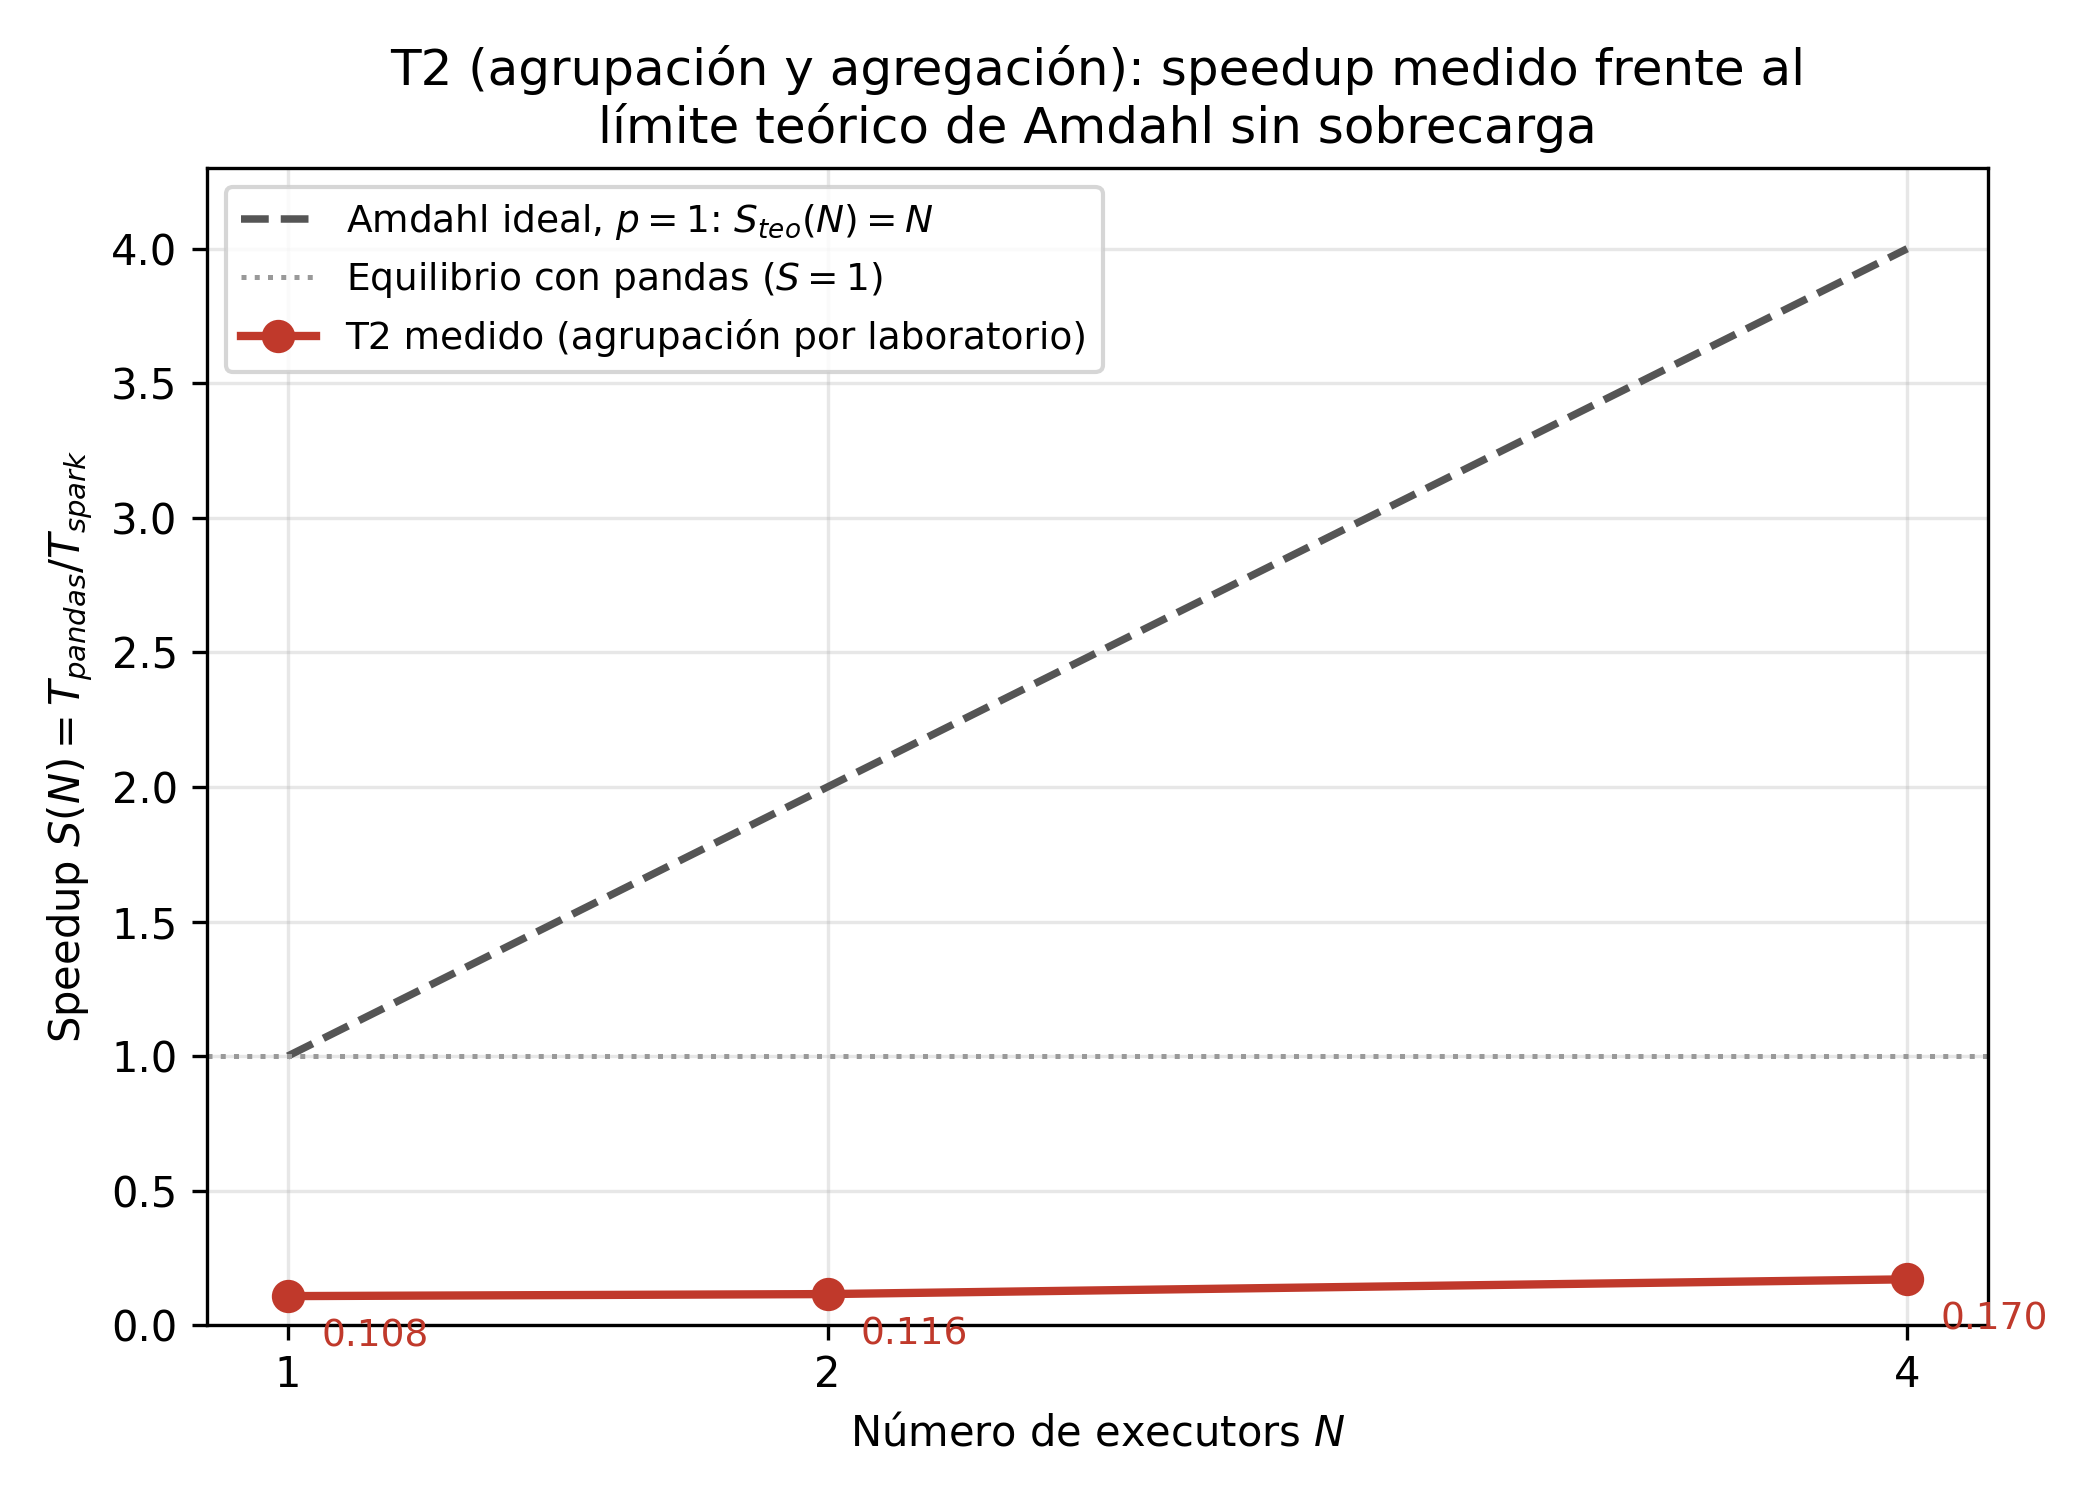
\includegraphics[width=\columnwidth]{../figuras/fig_speedup.png}
\caption{Speedup medido de T2 (agrupaci\'on por laboratorio) frente a la cota
superior te\'orica de Amdahl con $p=1$. La l\'inea punteada horizontal marca
el equilibrio con pandas ($S=1$); el speedup medido nunca la alcanza.
Figura de elaboraci\'on propia, \num{300} DPI, generada con matplotlib a
partir de \texttt{tiempos\_resumen.csv} del commit \texttt{a5ffcd9}.}
\label{fig:speedup}
\end{figure}

La desviaci\'on relativa se calcula como
$\Delta(N) = \bigl(S_{\text{med}}(N) - S_{\text{teo}}(N)\bigr)/S_{\text{teo}}(N)$,
expresada en porcentaje. Con $S_{\text{teo}}(N)=N$:
\begin{align}
\Delta(1) &= \frac{0.1080 - 1}{1} = -\SI{89.20}{\percent},\\
\Delta(2) &= \frac{0.1155 - 2}{2} = -\SI{94.23}{\percent},\\
\Delta(4) &= \frac{0.1704 - 4}{4} = -\SI{95.74}{\percent}.
\label{eq:desviacion}
\end{align}
La desviaci\'on no solo es negativa sino creciente en magnitud con $N$: cuanto
m\'as recursos se a\~naden, m\'as se aleja el sistema real de la cota ideal,
porque el numerador (speedup medido) crece de forma casi plana mientras el
denominador (cota te\'orica) crece linealmente.

\subsection{Respuesta expl\'icita: el caso $S<1$}
Los resultados de T2 \textbf{no coinciden} con la predicci\'on de Amdahl bajo
ninguna configuraci\'on medida: el speedup permanece por debajo de la unidad
en $N=1$, $N=2$ y $N=4$, es decir, la versi\'on distribuida es siempre m\'as
lenta que la versi\'on secuencial en pandas. La Ley de Amdahl, en su
formulaci\'on cl\'asica~\eqref{eq:amdahl}, no puede predecir este caso porque
se deriva bajo la hip\'otesis de sobrecarga nula: el \'unico costo que el
modelo reconoce es el de la fracci\'on estrictamente serial, y el \'unico
efecto de a\~nadir procesadores es acelerar la fracci\'on paralela. Un motor
distribuido real, en cambio, introduce un costo de coordinaci\'on --arranque
de sesi\'on, planificaci\'on del DAG, serializaci\'on y shuffle-- que el
modelo simplemente no representa~\cite{hillmarty2008}. Cuando ese costo de
coordinaci\'on por s\'i solo supera el tiempo total de la alternativa
secuencial, como ocurre aqu\'i, ning\'un valor de $p<1$ en la
ecuaci\'on~\eqref{eq:amdahl} puede producir $S<1$: el modelo est\'a, por
construcci\'on, fuera de su dominio de aplicaci\'on v\'alido para este caso.
Esta observaci\'on es exactamente la formalizada por Hill y Marty al
argumentar que, en arquitecturas multin\'ucleo y distribuidas reales, la ley
de Amdahl cl\'asica sistem\'aticamente sobreestima el rendimiento alcanzable
porque ignora los costos de sincronizaci\'on y comunicaci\'on que crecen con
$N$~\cite{hillmarty2008}.

% ----------------------------------------------------------------------------
\section{Diagn\'ostico de la fracci\'on no escalable}
\label{sec:diagnostico}

\subsection{M\'etrica de Karp-Flatt y su dominio de validez}
La m\'etrica de Karp-Flatt despeja, a partir del speedup observado $S$ con
$N$ unidades, la fracci\'on serial experimental
\begin{equation}
e = \frac{\dfrac{1}{S} - \dfrac{1}{N}}{1 - \dfrac{1}{N}}, \qquad N>1,
\label{eq:karpflatt}
\end{equation}
propuesta originalmente como diagn\'ostico de la porci\'on no paralelizable
de un c\'omputo real~\cite{karpflatt1990}. Sustituyendo los valores de la
Tabla~\ref{tab:escaladoT2}:
\begin{align}
e(2) &= \frac{\dfrac{1}{0.1155} - \dfrac{1}{2}}{1 - \dfrac{1}{2}}
       = \frac{8.6579 - 0.5}{0.5} = 16.316,\\
e(4) &= \frac{\dfrac{1}{0.1704} - \dfrac{1}{4}}{1 - \dfrac{1}{4}}
       = \frac{5.8697 - 0.25}{0.75} = 7.492.
\label{eq:karpflatt_num}
\end{align}
Ambos valores son mayores que $1$, lo cual es matem\'aticamente imposible
para una fracci\'on serial: por definici\'on, $e \in [0,1]$. Este no es un
error de c\'alculo, sino la consecuencia directa de que la
ecuaci\'on~\eqref{eq:karpflatt} es algebraicamente equivalente a despejar $p$
de~\eqref{eq:amdahl}, y por tanto hereda la misma hip\'otesis de sobrecarga
nula. Cuando $S<1$, como ocurre en las tres configuraciones de T2, la
f\'ormula produce un valor fuera de su dominio v\'alido: el resultado debe
interpretarse como una se\~nal de que el modelo de dos t\'erminos (fracci\'on
serial fija m\'as fracci\'on paralela perfectamente escalable) es inadecuado
para describir esta transformaci\'on, no como una fracci\'on serial real de
$1631\,\%$ o $749\,\%$.

\subsection{Lectura de la tendencia}
Aunque los valores individuales de $e$ carecen de significado como fracci\'on,
su \textbf{tendencia} s\'i es informativa: $e$ \emph{disminuye} de $16.316$ en
$N=2$ a $7.492$ en $N=4$, es decir, a la inversa que si la sobrecarga
creciera con el n\'umero de executors (lo que se manifestar\'ia como $e$
creciente, seg\'un el criterio de interpretaci\'on est\'andar de la
m\'etrica). La disminuci\'on observada es consistente con una interpretaci\'on
espec\'ifica: el costo dominante en T2 es un costo \textbf{fijo} por
ejecuci\'on (arranque de la sesi\'on Spark, planificaci\'on del plan f\'isico,
apertura de conexiones entre executors), no un costo que crezca con $N$; al
aumentar $N$, ese costo fijo se diluye levemente porque el shuffle en s\'i se
paraleliza entre m\'as executors, lo que hace que $S(N)$ crezca muy poco
(de $0.108$ a $0.170$) y, en consecuencia, que el valor calculado de $e$
--que depende inversamente de $S$-- disminuya. La lectura correcta no es
``el algoritmo escala mal'' ni ``la sobrecarga crece con $N$'', sino que
\textbf{el costo de coordinaci\'on fijo del motor es, por s\'i solo, mayor que
todo el presupuesto de tiempo de la alternativa secuencial}, independientemente
de $N$.

\subsection{Atribuci\'on a mecanismos concretos}
Se identifican tres mecanismos concretos, no gen\'ericos, que explican la
sobrecarga de T2, cada uno vinculado a evidencia propia verificable en el
repositorio (no a una Spark UI capturada espec\'ificamente para T2, que no
forma parte de la evidencia de PE-U4, sino a las salidas de datos y a las
mediciones ya reportadas):
\begin{enumerate}
\item \textbf{Shuffle desproporcionado al resultado \'util.} T2 agrupa
\num{500000} filas de solicitudes en solo 40 grupos de salida (uno por
laboratorio). El motor debe redistribuir por red la totalidad de las filas de
entrada antes de poder aplicar la agregaci\'on, aun cuando el resultado final
es min\'usculo. \emph{Evidencia propia:} la salida persistida
\texttt{data/spark/T2\_agrupacion/} del repositorio de PE-U4 se escribe en una
\'unica partici\'on de archivo, frente a las dos particiones que exhiben las
salidas de T1, T3 y T4; el resultado final de T2 es tan peque\~no que ni
siquiera justifica m\'as de un archivo de salida, lo que contrasta
directamente con el volumen que debi\'o moverse por la red durante el
shuffle previo. Yu et al. documentan que la operaci\'on de
reducci\'on/agregaci\'on en Spark es el cuello de botella de escalabilidad
menos favorable del motor cuando el volumen de datos movidos por el shuffle
no guarda proporci\'on con el trabajo \'util de reducci\'on
posterior~\cite{sparker2021}.
\item \textbf{Arranque y planificaci\'on de sesi\'on.} Cada configuraci\'on de
$N$ se midi\'o con una sesi\'on Spark Standalone independiente, seg\'un el
protocolo de PE-U4; el establecimiento de la conexi\'on con el cl\'uster, el
registro de executors y la construcci\'on del plan f\'isico por el
optimizador Catalyst introducen un costo fijo por ejecuci\'on que no existe en
pandas. \emph{Evidencia propia:} con un \'unico executor ($N=1$, sin ning\'un
costo de coordinaci\'on \emph{entre} executors posible), T2 en PySpark ya
mide \SI{1.0850}{\second} frente a \SI{0.1171}{\second} de pandas
(Tabla~\ref{tab:escaladoT2}), una raz\'on de $9.27\times$; puesto que con un
solo executor no hay comunicaci\'on inter-nodo que explicar, esa brecha
completa es atribuible al costo fijo de sesi\'on y planificaci\'on, no a la
coordinaci\'on entre m\'ultiples executors~\cite{zaharia2016}.
\item \textbf{Ausencia de agregaci\'on parcial efectiva a esta cardinalidad.}
\emph{Evidencia propia:} la verificaci\'on de equivalencia del notebook de
PE-U4 confirma que la salida de T2 tiene exactamente 40 filas, id\'enticas
entre pandas y PySpark. Con solo 40 claves de salida, la etapa de
reducci\'on posterior al shuffle es casi instant\'anea; todo el tiempo de la
transformaci\'on distribuida se concentra en mover datos, no en calcularlos,
de modo que a\~nadir executors divide el trabajo de shuffle entre m\'as
unidades sin reducir el volumen
total transferido por la red.
\end{enumerate}

% ----------------------------------------------------------------------------
\section{Propuesta de integraci\'on al PFC}
\label{sec:propuesta}

\subsection{Caso de uso}
En el SCLI, el proceso an\'alogo a T2 es la generaci\'on peri\'odica de un
\textbf{reporte de demanda por laboratorio}: agrupar las solicitudes de
reserva registradas en un per\'iodo, contar cu\'antas corresponden a cada
laboratorio y calcular la ocupaci\'on promedio y m\'axima. La salida de este
reporte alimenta una decisi\'on operativa concreta: la
\textbf{reprogramaci\'on de mantenimiento preventivo y la reasignaci\'on de
cupos de horario} hacia los laboratorios con mayor demanda sostenida,
decisi\'on que hoy en el SCLI se toma sin ese insumo cuantitativo.

\subsection{Periodicidad y volumen}
A diferencia de una consulta transaccional (por ejemplo, verificar
disponibilidad al momento de reservar), este reporte no requiere latencia baja:
tiene sentido ejecutarlo por lotes, con periodicidad \textbf{semanal}
(coincidente con el ciclo de planificaci\'on acad\'emica) o, como m\'inimo,
mensual. El volumen actual estimado de solicitudes por semestre en un
despliegue real de la Facultad es de algunos miles a pocas decenas de miles de
registros --muy por debajo del umbral de rentabilidad calculado en la
Secci\'on~\ref{sec:dimensionamiento}--, aunque el volumen acumulado
hist\'orico crece con cada per\'iodo acad\'emico.

\subsection{Arquitectura de integraci\'on}
La Fig.~\ref{fig:arquitectura} muestra el punto exacto de inserci\'on en la
arquitectura en capas del SCLI. El procesamiento se ejecuta \textbf{por
lotes}, no en flujo: un planificador (por ejemplo, un \textit{cron job} o un
DAG de Airflow) dispara semanalmente un job de agregaci\'on que lee de la capa
de datos operacional (la tabla \texttt{solicitudes\_reserva} de PostgreSQL),
calcula la agregaci\'on por laboratorio y escribe el resultado en una capa de
\emph{reporting} separada (una tabla o vista materializada
\texttt{demanda\_laboratorio}), que a su vez alimenta el panel de
coordinaci\'on consumido por la capa de presentaci\'on. El job de agregaci\'on
nunca escribe sobre la base operacional, de modo que un fallo o una demora en
el reporte no compromete la disponibilidad del sistema transaccional de
reservas.

\begin{figure}[!t]
\centering
\begin{tikzpicture}[
  node distance=0.55cm and 1.0cm,
  capa/.style={rectangle, draw, rounded corners, minimum width=6.6cm,
               minimum height=0.85cm, align=center, font=\scriptsize},
  proceso/.style={rectangle, draw, rounded corners, minimum width=6.6cm,
               minimum height=0.85cm, align=center, font=\scriptsize,
               fill=black!8},
  flecha/.style={-{Latex[length=2mm]}, thick}
]
\node[capa] (presentacion) {Capa de presentaci\'on\\ Panel de coordinaci\'on del SCLI (web)};
\node[capa, below=of presentacion] (reporting) {Capa de \textit{reporting}\\ Vista \texttt{demanda\_laboratorio} (PostgreSQL)};
\node[proceso, below=of reporting] (batch) {Job de agregaci\'on por lotes\\ (an\'alogo a T2: agrupaci\'on por laboratorio)};
\node[capa, below=of batch] (operacional) {Capa de datos operacional\\ \texttt{solicitudes\_reserva}, \texttt{laboratorios}};

\draw[flecha] (operacional) -- (batch);
\draw[flecha] (batch) -- (reporting);
\draw[flecha] (reporting) -- (presentacion);

\node[left=0.3cm of batch, font=\scriptsize, align=center, text width=1.6cm]
  (scheduler) {Planificador\\ semanal\\ (cron / Airflow)};
\draw[flecha] (scheduler) -- (batch);
\end{tikzpicture}
\caption{Punto de inserci\'on del procesamiento por lotes en la arquitectura
en capas del SCLI. El job se dispara semanalmente, lee de la capa
operacional y escribe exclusivamente en una capa de \textit{reporting}
aislada, sin afectar la disponibilidad transaccional. Diagrama de
elaboraci\'on propia (TikZ).}
\label{fig:arquitectura}
\end{figure}

% ----------------------------------------------------------------------------
\section{Dimensionamiento y viabilidad}
\label{sec:dimensionamiento}

\subsection{Umbral de rentabilidad}
Modelando el tiempo secuencial como $T_{\text{sec}}(n) = \alpha n$ y el
distribuido como $T_{\text{dist}}(n) = \beta + \gamma n / N$, donde $\beta$
agrupa la sobrecarga fija y $n$ es el n\'umero de registros, el motor
distribuido resulta ventajoso cuando $T_{\text{dist}}(n) < T_{\text{sec}}(n)$,
es decir:
\begin{equation}
n^{*} = \frac{\beta}{\alpha - \dfrac{\gamma}{N}}, \qquad \text{v\'alido si } \alpha > \frac{\gamma}{N}.
\label{eq:umbral}
\end{equation}
Los par\'ametros se estimaron por regresi\'on lineal de m\'inimos cuadrados
sobre las tres mediciones propias de T2 ($N=1,2,4$, con $n=\num{500000}$
fijo), tomando $x=1/N$ como variable independiente:
$\alpha = T_{\text{pandas}}/n = \num{2.3427e-7}\,\si{\second}$ por registro;
$\beta = \SI{0.6521}{\second}$ (ordenada al origen del ajuste); y
$\gamma = \num{9.4903e-7}\,\si{\second}$ por registro (pendiente del ajuste
dividida entre $n$).

Sustituyendo en la condici\'on de validez de~\eqref{eq:umbral} con $N=4$, la
configuraci\'on usada en PE-U4:
\begin{equation}
\alpha - \frac{\gamma}{4} = \num{2.3427e-7} - \num{2.3726e-7} = \num{-2.99e-9} < 0.
\label{eq:umbral_n4}
\end{equation}
La condici\'on \textbf{no se cumple}: con $N=4$ executors, el costo marginal
por registro del motor distribuido es, por muy poco, mayor que el de pandas.
Bajo este modelo lineal, \textbf{no existe ning\'un volumen finito} de datos
que rentabilice Spark para T2 con esa configuraci\'on de cl\'uster --el umbral
$n^{*}$ diverge--. Despejando el $N$ m\'inimo para el cual la condici\'on se
satisface, $N^{*} = \gamma/\alpha \approx 4.05$: el punto de equilibrio est\'a
justo por encima de los cuatro executors usados en la pr\'actica. La
Tabla~\ref{tab:nstar} extrapola $n^{*}$ para configuraciones mayores, fuera
del rango medido, declarando expl\'icitamente esa extrapolaci\'on como
limitaci\'on del ajuste.

\begin{table}[!t]
\centering
\footnotesize
\caption{Umbral de rentabilidad $n^{*}$ extrapolado para $N>4$ (fuera del
rango medido; el modelo solo fue ajustado con $N=1,2,4$).}
\label{tab:nstar}
\begin{tabular}{@{}S[table-format=2.0]S[table-format=8.0]@{}}
\toprule
{$N$ (executors)} & {$n^{*}$ (registros)}\\
\midrule
5  & 14\,665\,148\\
8  & 5\,638\,763\\
16 & 3\,727\,083\\
\bottomrule
\end{tabular}
\end{table}

\subsection{Modelo de servicio en la nube}
Dado que el volumen proyectado del SCLI (Secci\'on~\ref{sec:propuesta}) est\'a
muy por debajo de cualquier $n^{*}$ de la Tabla~\ref{tab:nstar}, mantener un
cl\'uster Spark permanente ser\'ia un sobredimensionamiento. Se recomienda un
modelo \textbf{PaaS con aprovisionamiento el\'astico bajo demanda}
--equivalente a un servicio gestionado tipo EMR/HDInsight/Dataproc-- que solo
se instancia si, en el futuro, el volumen supera el umbral calculado; esto
aprovecha la caracter\'istica de elasticidad r\'apida del c\'omputo en la
nube~\cite{mell2011} sin incurrir en el costo fijo de un cl\'uster ocioso la
mayor parte del tiempo. Mientras el volumen se mantenga por debajo del umbral,
el job de agregaci\'on de la Fig.~\ref{fig:arquitectura} debe ejecutarse
directamente sobre la base de datos operacional (Secci\'on~\ref{sec:postura}).

\subsection{Recursos y riesgos}
Los recursos requeridos bajo el modelo recomendado son m\'inimos: el mismo
servidor que aloja PostgreSQL puede ejecutar la consulta de agregaci\'on
peri\'odica sin infraestructura adicional. El principal riesgo identificado es
de \textbf{validez del modelo}: $\alpha$, $\beta$ y $\gamma$ se estimaron sobre
un conjunto sint\'etico y con solo tres puntos de medici\'on; el umbral debe
recalcularse cuando existan mediciones sobre datos reales de producci\'on del
SCLI, y la extrapolaci\'on de la Tabla~\ref{tab:nstar} para $N>4$ debe tratarse
como orientativa hasta que se mida directamente.

% ----------------------------------------------------------------------------
\section{Postura cr\'itica y alternativas}
\label{sec:postura}

Con la evidencia de las secciones anteriores, la postura de este informe es
que \textbf{Spark no es la opci\'on correcta} para el reporte de demanda por
laboratorio del SCLI en su estado actual: el speedup medido es inferior a 1
en toda la escala evaluada, la condici\'on de rentabilidad de la
ecuaci\'on~\eqref{eq:umbral} no se satisface con la configuraci\'on de
cl\'uster disponible, y el volumen proyectado del sistema est\'a muy por
debajo de cualquier umbral extrapolado razonable. Esta conclusi\'on es
consistente con el argumento de McSherry et al., quienes muestran que
numerosos sistemas de macrodatos publicados requieren cientos de n\'ucleos
antes de superar el desempe\~no de una implementaci\'on de un solo hilo bien
escrita, y que la escalabilidad por s\'i sola --sin comparar contra ese
punto de referencia-- es una m\'etrica enga\~nosa~\cite{mcsherry2015}.

Se evaluaron y descartaron dos alternativas distribuidas antes de llegar a la
recomendaci\'on final:
\begin{itemize}
\item \textbf{Dask.} Ofrece una API similar a pandas con ejecuci\'on
distribuida y podr\'ia reducir la curva de aprendizaje frente a PySpark. Se
descarta porque su operaci\'on \texttt{groupby} sobre claves de baja
cardinalidad exhibe el mismo patr\'on de shuffle completo que Spark: el
problema de fondo (movimiento de datos desproporcionado al resultado) no es
espec\'ifico del motor, sino de la operaci\'on, y a\~nadir un planificador
distribuido introducir\'ia complejidad operativa sin resolver la causa ra\'iz.
\item \textbf{Almac\'en de datos anal\'itico gestionado en la nube} (por
ejemplo, un servicio tipo BigQuery o Redshift). Se descarta por
desproporci\'on: el costo recurrente y el bloqueo de proveedor no se
justifican para un reporte semanal sobre un volumen de datos que cabe
c\'omodamente en una \'unica tabla indexada de PostgreSQL.
\end{itemize}
La alternativa recomendada --ya integrada en la Fig.~\ref{fig:arquitectura}--
es ejecutar la agregaci\'on directamente como una consulta \texttt{GROUP BY}
indexada sobre la base operacional del SCLI, revalidando peri\'odicamente el
umbral $n^{*}$ a medida que el sistema acumula historial. Esta postura no es
definitiva: si el SCLI evolucionara hacia un volumen de solicitudes
multi-institucional, o si el mecanismo de agregaci\'on cambiara para reducir
el shuffle (por ejemplo, mediante agregaci\'on parcial en el lado del mapa),
la conclusi\'on deber\'ia revisarse.

% ----------------------------------------------------------------------------
\section{Conclusiones}
\label{sec:conclusiones}

\begin{enumerate}
\item El speedup de T2 result\'o inferior a la unidad en las tres
configuraciones medidas ($0.108$, $0.116$ y $0.170$ para $N=1,2,4$), un caso
que la Ley de Amdahl cl\'asica no puede predecir por estar fuera de su
hip\'otesis de sobrecarga nula~\cite{amdahl1967,hillmarty2008}; esta evidencia
muestra en la pr\'actica que un motor distribuido introduce un costo de
coordinaci\'on que ninguna cantidad de paralelismo algor\'itmico compensa
cuando el resultado \'util es peque\~no frente al volumen de entrada.

\item La m\'etrica de Karp-Flatt, calculada sobre los datos propios de T2,
arroj\'o valores fuera de su dominio v\'alido ($e(2)=16.32$, $e(4)=7.49$), lo
que --lejos de ser un error-- constituye evidencia diagn\'ostica de que el
modelo de dos t\'erminos que sustenta tanto a Amdahl como a Karp-Flatt es
inadecuado para transformaciones dominadas por un costo fijo de
coordinaci\'on, como el shuffle de baja cardinalidad de
T2~\cite{karpflatt1990,sparker2021}.

\item El ajuste del modelo de umbral de rentabilidad sobre las mediciones
propias mostr\'o que, con la configuraci\'on de cl\'uster de PE-U4 ($N=4$),
ning\'un volumen de datos hace rentable a Spark para esta operaci\'on, y que
se requieren al menos cinco executors para que el umbral vuelva a ser finito;
esta cifra, aplicada al SCLI, respalda una decisi\'on de arquitectura
concreta: mantener la agregaci\'on de demanda por laboratorio en la base de
datos operacional en lugar de introducir un motor distribuido de forma
prematura.
\end{enumerate}

% ----------------------------------------------------------------------------
\section{Declaraci\'on de uso de inteligencia artificial generativa}
\label{sec:ia}

Se emplearon dos herramientas de inteligencia artificial generativa en la
elaboraci\'on de este informe. \textbf{Claude (Anthropic)} asisti\'o en: la
redacci\'on y estructuraci\'on del documento LaTeX conforme a la gu\'ia
TA-IND-04; el c\'alculo de la regresi\'on lineal de m\'inimos cuadrados para
estimar $\alpha$, $\beta$ y $\gamma$ de la ecuaci\'on~\eqref{eq:umbral}; la
generaci\'on del script de la Fig.~\ref{fig:speedup} con matplotlib; la
verificaci\'on de las referencias bibliogr\'aficas y sus DOI; y la redacci\'on
del diagrama TikZ de la Fig.~\ref{fig:arquitectura}. \textbf{Codex (OpenAI)}
asisti\'o en la auditor\'ia de solo lectura del repositorio de PE-U4 y en la
ejecuci\'on del protocolo de medici\'on de T2 con $N=1$ y $N=2$ executors,
replicando exactamente el protocolo ya usado por el equipo para $N=4$. Todo
el an\'alisis cuantitativo, la interpretaci\'on de los resultados, la
propuesta de integraci\'on al PFC y las conclusiones son de autor\'ia y
responsabilidad del estudiante. Se declara adem\'as que la medici\'on de T2
con $N=1$ y $N=2$ no exist\'ia en el commit original de PE-U4 --la gu\'ia
grupal solo exig\'ia ese escalado para T3-- y fue generada expresamente para
este informe individual, incorpor\'andose al repositorio grupal en el commit
\texttt{bbe19c8} para preservar la trazabilidad exigida.

% ----------------------------------------------------------------------------
\printbibliography

\end{document}
